\begin{figure}[h]
    \centering
    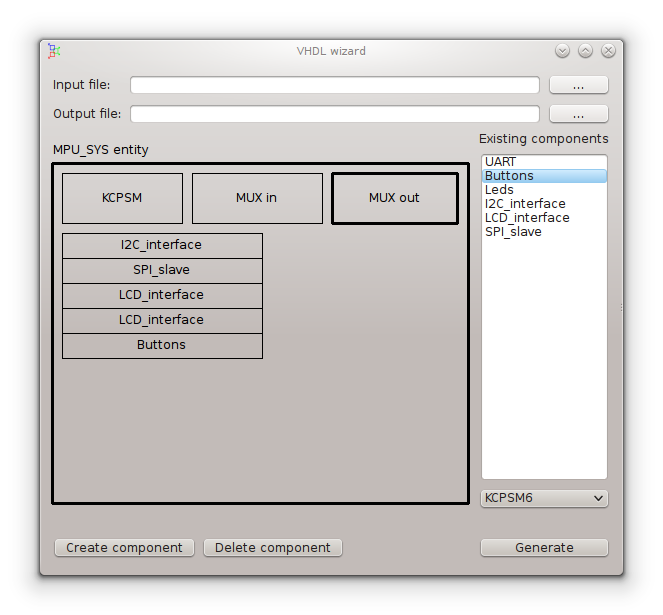
\includegraphics[width=.5\textwidth]{img/VHDL_wizard.png}
    \caption{VHDL Wizard}
\end{figure}

\subsubsection{Purpose of this tool}
    TEMPLATE
    This tool will automaticaly generate VHDL code for quicker connection of your picoblaze design with your VHDL design. It will take
    PORTs declared in your assembler design and generates appropriate constants and input/output multiplexers.

\subsubsection{Main window}
    \begin{description}
        \item [Input file]
            Select path to your .stbl(symbol table) file generated after the compilation of you assembler source code. Note, make sure you
            have generation of the file allowed (Project->Configure->Compiler->Options->Symbol table checked).
        \item [Output file]
            Select path of your generated file, which contains generated VHDL template.
        \item [MPU\_SYS entity]
            General look to your template entity. Every box symbolise vhdl component. There are always three default boxes. KCPSM component, Input demux.
            and output mux. You can click to every one of them for detail info. When you create or add some custom component, it will show
            up here.
        \item [Existing components]
            This list contains all your previously defined components.
        \item [KCPSM combobox]
            With this compobox you can select KCPSM version of your picoblaze design. It will change the declaration and instantiation of picoblaze
            in generated vhdl file. KCPSM6 is selected by default.
        \item [Create component button]
            This button will open create component dialog where you can define you new component. See the next section "Create component dialog".
        \item [Delete component button]
            This button will remove one component from your MPU\_SYS entity.
        \item [Generate]
            If you have your input and output file selected. This button will trigger generation of VHDL template.
    \end{description}

\subsubsection{Create component dialog}
    With this dialog, you can define your custom component and add it to the generated template. 
    \begin{description}
        \item [Component name]
            Name of your component.
        \item [Tab port and generic]
            Port tab lets you define component ports
        \item [Port name/ Generic name]
            Name of evvery port or generic.
        \item [Value]
            You can set initial value. Leaving this field empty means no initial value is needed.
        \item [Direction/Type]
            Direction in port tab can be IN,OUT or INOUT. In generic tab, you define type of your generic attribute. Logic means zero or one. Logic vector is bus, define with MSB and LSB numbers.
            Integer can be number defined from range -2147483648 to +2147483647. Positive is RANGE 1 TO integer’HIGH. Natural is in RANGE 0 TO integer’HIGH.
        \item [Bus check-box]
            Telling generator that you
        \item [Signal/Constant check-box]
            If checked, generator will insert this port or attribute declared as signal or constant in VHDL template.
        \item [Generate]
            If you have your input and output file selected. This button will trigger generation of VHDL template.
    \end{description}

\begin{figure}[h]
    \centering
    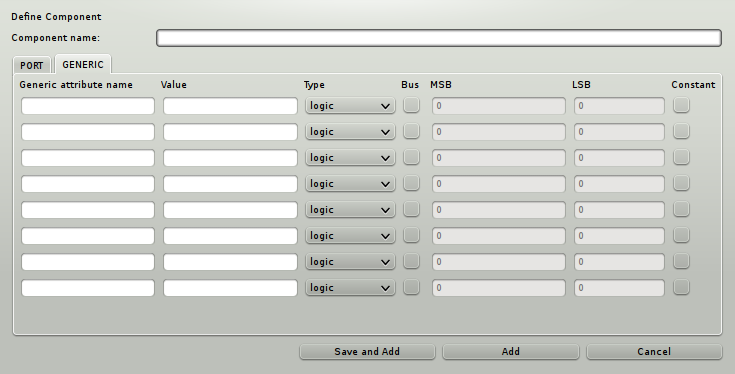
\includegraphics[width=.5\textwidth]{img/VHDL_create_generic.png}
    \caption{Custom component generic parameters}
\end{figure}

\begin{figure}[h]
    \centering
    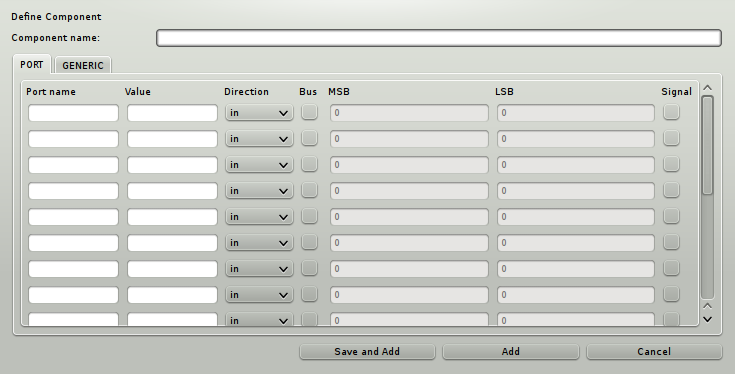
\includegraphics[width=.5\textwidth]{img/VHDL_create_component.png}
    \caption{VHDL Wizard}
\end{figure}


\subsubsection{Create component dialog}
    Phasellus sit amet quam nec nulla euismod dignissim. Fusce ante felis, tincidunt nec egestas id, interdum a magna. Curabitur felis nisl, placerat quis ex eget, iaculis eleifend tellus. Praesent finibus ac mauris feugiat consequat. Praesent a faucibus quam, quis fermentum felis. Nam porta tellus sed eros blandit viverra. In rhoncus viverra mi et varius. Morbi sodales egestas sollicitudin. Pellentesque euismod risus id magna posuere, et mattis mi dictum. Pellentesque habitant morbi tristique senectus et netus et malesuada fames ac turpis egestas. Vestibulum ullamcorper tortor eget lectus ultricies ultricies. Aliquam in nunc ac tortor pellentesque sodales. Nullam posuere sollicitudin ligula quis condimentum. Maecenas dolor orci, tempor non tristique id, aliquet eget eros. Praesent malesuada facilisis lacus a vulputate.

\subsubsection{Examples}
    Quisque fermentum ligula augue, id ullamcorper libero auctor vulputate. Mauris mollis velit leo, in scelerisque lorem maximus ut. Proin vehicula libero nec odio sagittis, vel tempor ante imperdiet. Suspendisse dui neque, luctus ac pretium vulputate, porttitor at lectus. Fusce sem sapien, semper eu faucibus a, cursus nec diam. Aliquam accumsan metus sed odio dapibus, eget vulputate felis pretium. Proin ut lorem vel elit ultrices commodo. Donec vitae finibus ex.